\documentclass[a4paper,14pt]{extarticle}

\usepackage[utf8x]{inputenc}
\usepackage[T1,T2A]{fontenc}
\usepackage[russian]{babel}
\usepackage{hyperref}
\usepackage{indentfirst}
\usepackage{here}
\usepackage{array}
\usepackage{graphicx}
\usepackage{caption}
\usepackage{subcaption}
\usepackage{chngcntr}
\usepackage{amsmath}
\usepackage{amssymb}
\usepackage{pgfplots}
\usepackage{pgfplotstable}
\usepackage[left=2cm,right=2cm,top=2cm,bottom=2cm,bindingoffset=0cm]{geometry}
\usepackage{multicol}
\usepackage{askmaps}
\usepackage{enumitem}

\setitemize{itemsep=0em}
\setenumerate{itemsep=0em}

\renewcommand{\le}{\ensuremath{\leqslant}}
\renewcommand{\leq}{\ensuremath{\leqslant}}
\renewcommand{\ge}{\ensuremath{\geqslant}}
\renewcommand{\geq}{\ensuremath{\geqslant}}
\renewcommand{\epsilon}{\ensuremath{\varepsilon}}
\renewcommand{\phi}{\ensuremath{\varphi}}
\renewcommand{\thefigure}{\arabic{figure}} 	
\renewcommand*\not[1]{\overline{#1}}

%\titleformat*{\section}{\large\bfseries} 
%\titleformat*{\subsection}{\normalsize\bfseries} 
%\titleformat*{\subsubsection}{\normalsize\bfseries} 
%\titleformat*{\paragraph}{\normalsize\bfseries} 
%\titleformat*{\subparagraph}{\normalsize\bfseries} 

\counterwithin{figure}{section}
\counterwithin{equation}{section}
\counterwithin{table}{section}
\newcommand{\sign}[1][5cm]{\makebox[#1]{\hrulefill}}
\graphicspath{{../pics/}}
\captionsetup{justification=centering,margin=1cm}
\def\arraystretch{1.3}
\setlength\parindent{5ex}
%\titlelabel{\thetitle.\quad}

\begin{document}

\begin{titlepage}
\begin{center}
	Санкт-Петербургский Политехнический Университет Петра Великого\\[0.3cm]
	Институт компьютерных наук и технологий \\[0.3cm]
	Кафедра компьютерных систем и программных технологий\\[4cm]
	
	\textbf{ОТЧЕТ}\\ 
	\textbf{по лабораторной работе}\\[0.5cm]
	\textbf{<<Исследование персептронов>>}\\[0.1cm]
	\textbf{Нейроинформатика}\\[4.0cm]
\end{center}

\begin{flushright}
	\begin{minipage}{0.45\textwidth}
		\textbf{Работу выполнил студент}\\[3mm]
		группа 33501/4 \hspace*{10mm} Дьячков В.В.\\[5mm]
		\textbf{Преподаватель}\\[5mm]
		\sign[1.7cm] \hspace*{1mm} к.т.н., доц. Никитин К.В. \\[5mm]
	\end{minipage}
\end{flushright}

\vfill

\begin{center}
	Санкт-Петербург\\
	\the\year
\end{center}
\end{titlepage}

\addtocounter{page}{1}

\tableofcontents
\newpage
\listoffigures
\newpage

\section{Цели работы}

\begin{itemize}
	\setlength\itemsep{0em}
	\item Научиться формировать выборки, состоящие из обучающих и тестовых примеров
	для решения типовых задач классификации, аппроксимации.
	\item Овладеть навыками визуализации данных на плоскости при решении задач
	классификации и аппроксимации.
	\item Научиться рассчитывать основные показатели качества распознавания и
	представлять полученные результаты в табличной и графической формах.
\end{itemize}

\section{Крестики-нолики}

\subsection{Задание 1}

Разделим таблицу $4\times 4$ на крестики и нолики так, чтобы классы <<O>> и <<X>> были линейно неразделимы:
\begin{equation*}
\begin{cases}
	y = f(X)\\
	X = [x_1, x_2]\\
	x_i \in \{1, 2, 3, 4\}\\
	y_i \in \{0, 1\}
\end{cases}
\end{equation*}

\subsection{Задание 2}

На рис. \ref{fig:tic-tac-toe} изображен полученный пример.

\begin{figure}[H]
\begin{center}
	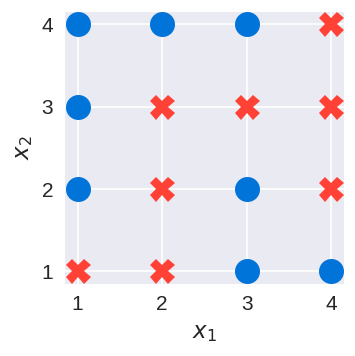
\includegraphics{1}
	\caption{Крестики-нолики}
	\label{fig:tic-tac-toe}
\end{center}
\end{figure}

\section{Логическая функция 5 переменных}

Зададим логическую функцию 5 переменных так, чтобы множество ее выходных значений 0 и 1 было линейно неразделимым:
\begin{equation*}
\begin{cases}
	y = f(X)\\
	X = [x_1, x_2, x_3, x_4, x_5]\\
	x_i \in \{0, 1\}\\
	y_i \in \{0, 1\}
\end{cases}
\end{equation*}

\vspace{-0.5cm}
\begin{table}[H]
\begin{center}
	\caption{Таблица истинности}
	\def\tabcolsep{15pt}
	\def\arraystretch{0.9}
	\pgfplotstabletypeset[col sep=comma,
	    columns={x1, x2, x3, x4, x5, y},
	    column type/.add={|c|}{},
	    columns/x1/.style={column name={$x_1$}},
	    columns/x2/.style={column name={$x_2$}},
	    columns/x3/.style={column name={$x_3$}},
	    columns/x4/.style={column name={$x_4$}},
	    columns/x5/.style={column name={$x_5$}},
	    columns/y/.style={column name={$y$}},
	    every head row/.style={before row=\hline, after row=\hline},
	    every last row/.style={after row=\hline}
	   ]{../data/truth_table.csv}
\end{center}
\end{table}

\section{Разбиение плоскости на 2 класса}

\subsection{Задание 1}

Разобьем прямоугольный участок плоскости с помощью отрезков прямых линий на два класса. На рис. \ref{fig:two_classes_plane_splitting} приведен графический эскиз полученного разбиения плоскости.

\subsection{Задание 2}

Сформируем матрицу входных значений $P$ в диапазоне рассматриваемого прямоугольного участка плоскости и найдем для нее вектор-столбец $T$, значения которого отвечают за номер класса (0 или 1). На рис. \ref{fig:two_classes_sample} изображена сформированная выборка, причем красным цветом отмечены значения, попадающие в область фигуры (1 класс).

\begin{figure}[H]
\begin{center}
	\begin{subfigure}[b]{0.49\textwidth}
		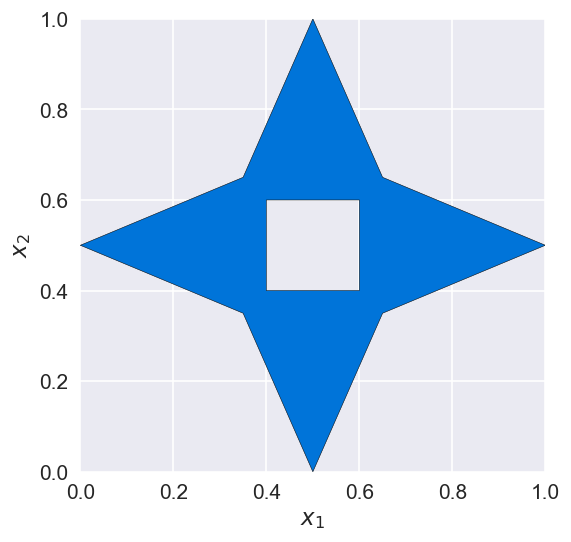
\includegraphics[width=\textwidth]{2}
		\caption{Разбиение плоскости}
		\label{fig:two_classes_plane_splitting}
	\end{subfigure}
	\begin{subfigure}[b]{0.49\textwidth}
		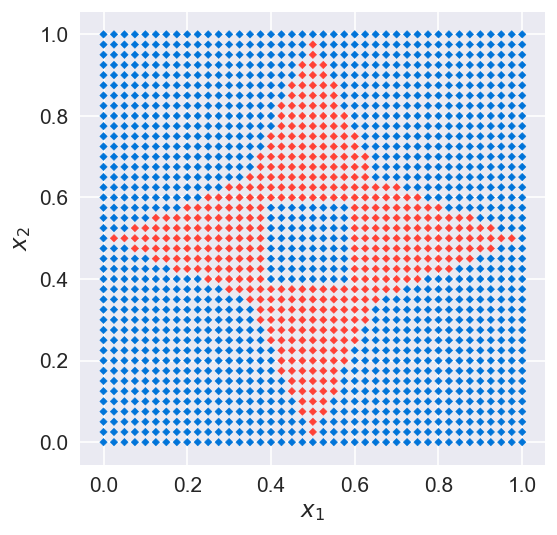
\includegraphics[width=\textwidth]{3}
		\caption{Выборка на плоскости}
		\label{fig:two_classes_sample}
	\end{subfigure}
	\caption{Разбиение и выбора на плоскости}
\end{center}
\end{figure}

\subsection{Задание 3}

Исказим сформированную ранее выборку $(P, T)$, проинвертировав значения 10\% случайно выбранных строк $T$, и будем интерпретировать эти данные, как ответ $Y$ некоторого распознающего устройства (классификатора). На рис. \ref{fig:two_classes_noise} изображена полученная выборка $(P, Y)$.

\begin{figure}[H]
\begin{center}
	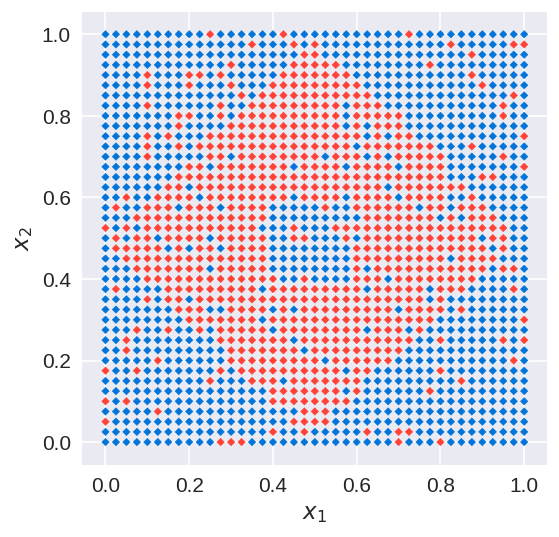
\includegraphics[scale=1]{4}
	\caption{Выборка, содержащая ошибки}
	\label{fig:two_classes_noise}
\end{center}
\end{figure}

На основании желаемых $T$ и реальных $Y$ ответов определим основные показатели качества распознавания. На рис. \ref{fig:two_classes_conf_matrix} изображена матрица неточностей.

\begin{figure}[H]
\begin{center}
	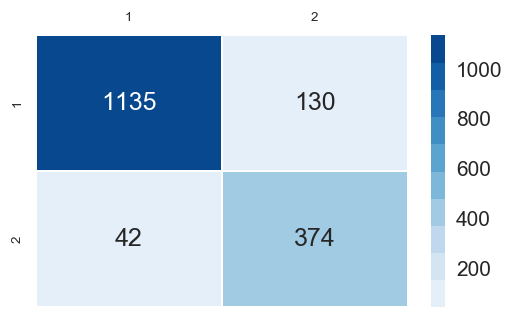
\includegraphics[scale=1]{5}
	\caption{Матрица неточностей}
	\label{fig:two_classes_conf_matrix}
\end{center}
\end{figure}

По значениям матрицы неточностей найдем другие характеристики классификации:
\begin{itemize}
	\setlength\itemsep{0em}
	\item Средняя вероятность ошибки: $\frac{130+42}{1681} = 0.10$
	\item Средняя вероятность правильного распознавания: $\frac{1118+391}{1681} = 0.90$
	\item Спецефичность: $\frac{1135}{1681} = 0.68$
	\item Чувствительность: = $\frac{374}{1681} = 0.22$
	\item Ошибка первого рода: = $\frac{130}{1681} = 0.08$
	\item Ошибка второго рода: = $\frac{42}{1681} = 0.02$
\end{itemize}

\subsection{Задание 4}

Разделим выборку на обучающую и тестовую, выбрав случайно $33\%$ примеров как тестовые, а остальные –- как обучающие. Полученное разделение изображено на рис. \ref{fig:two_classes_train_and_test}, причем большими точками отмечены примеры, попавшие в обучающую выборку, а маленькими -- в тестовую.

\begin{figure}[H]
\begin{center}
	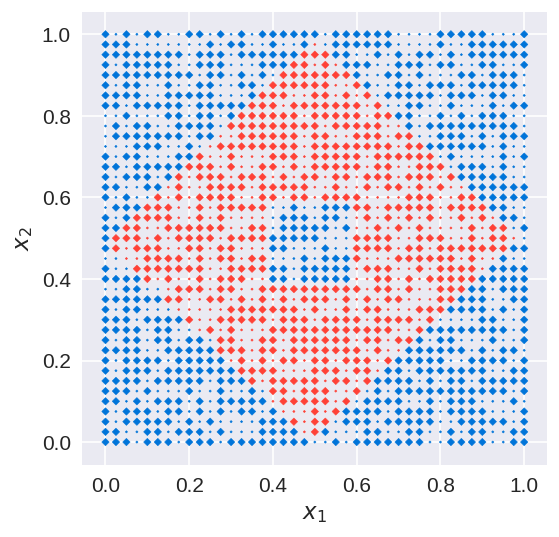
\includegraphics[scale=1]{6}
	\caption{Разделение выборки на обучающую и тестовую}
	\label{fig:two_classes_train_and_test}
\end{center}
\end{figure}

\newpage

Применим \textbf{K-fold} кросс-валидацию при $K=4$ к исходной выборке. Результат разбиения изображен на рис. \ref{fig:two_classes_kfold}, причем большими точками отмечены примеры, попавшие в обучающую выборку, а маленькими -- в тестовую.

\begin{figure}[H]
\begin{center}
	\begin{subfigure}[b]{0.49\textwidth}
		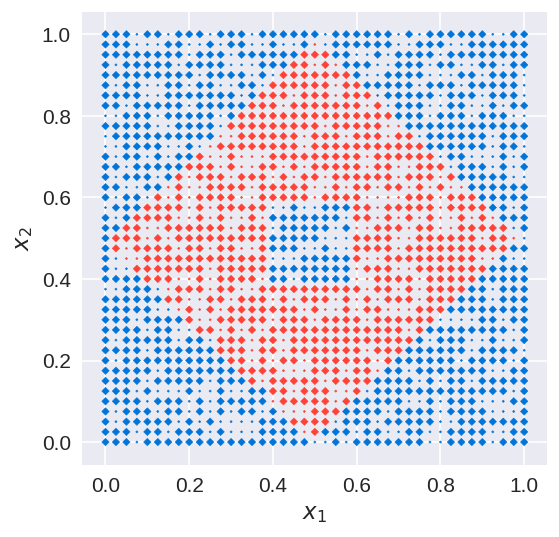
\includegraphics[width=\textwidth]{7}
	\end{subfigure}
	\begin{subfigure}[b]{0.49\textwidth}
		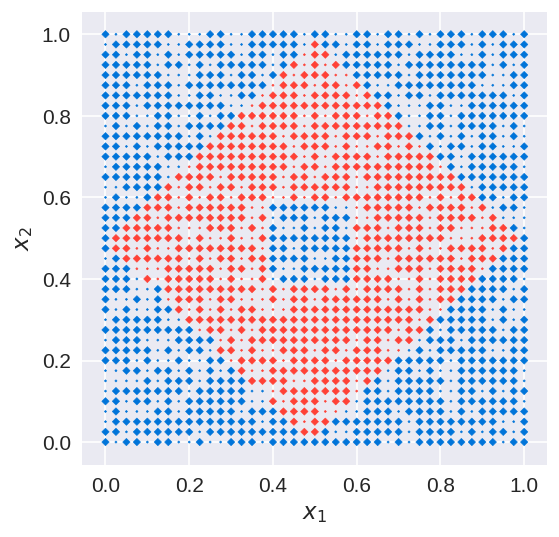
\includegraphics[width=\textwidth]{8}
	\end{subfigure}
	\begin{subfigure}[b]{0.49\textwidth}
		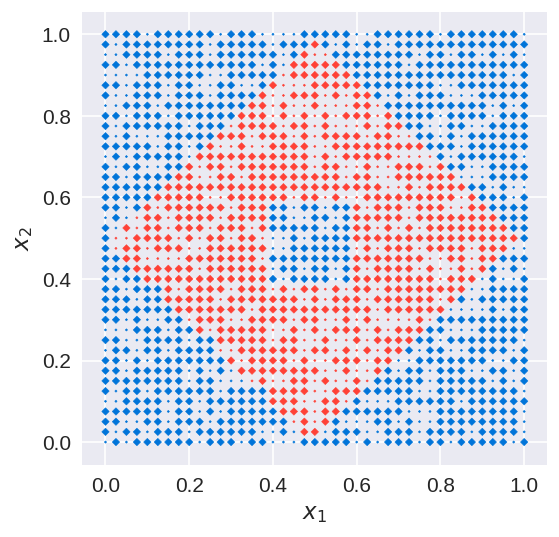
\includegraphics[width=\textwidth]{9}
	\end{subfigure}
	\begin{subfigure}[b]{0.49\textwidth}
		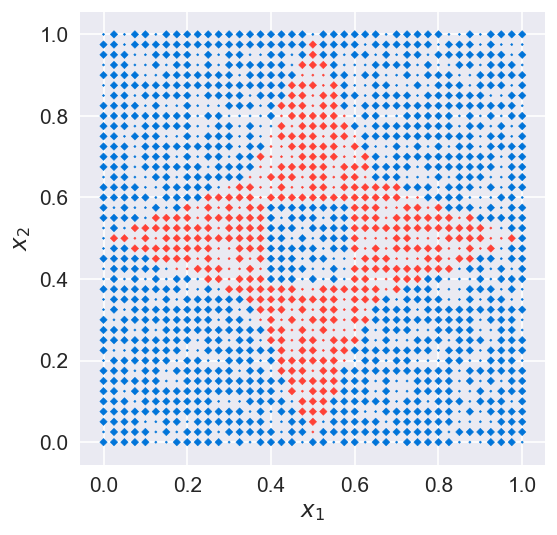
\includegraphics[width=\textwidth]{10}
	\end{subfigure}
	\caption{K-fold кросс-валидация}
	\label{fig:two_classes_kfold}
\end{center}
\end{figure}

\newpage

\section{Разбиение плоскости на N классов}

\subsection{Задание 1}

Разобьем прямоугольный участок плоскости с помощью отрезков прямых линий на 8 классов. На рис. \ref{fig:eight_classes_plane_splitting} приведен графический эскиз полученного разбиения плоскости.

\subsection{Задание 2}

Сформируем матрицу входных значений $P$ в диапазоне рассматриваемого прямоугольного участка плоскости и найдем для нее вектор-столбец $T$, значения которого отвечают за номер класса ($1,\dotsc ,8$). На рис. \ref{fig:eight_classes_sample} изображена сформированная выборка, причем разные классы отмечены разными цветами.

\begin{figure}[H]
\begin{center}
	\begin{subfigure}[b]{0.49\textwidth}
		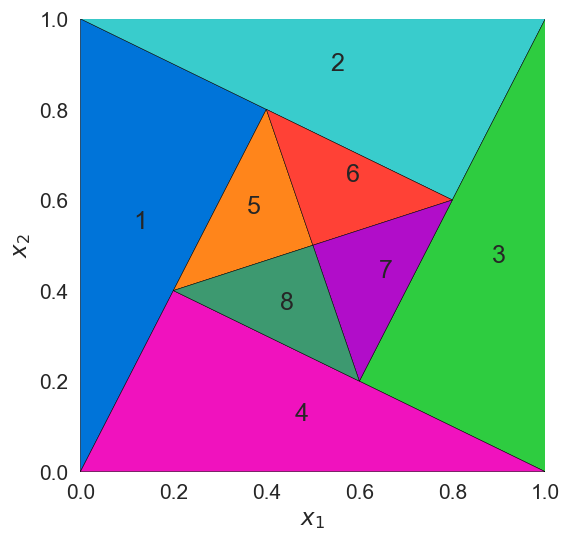
\includegraphics[width=\textwidth]{11}
		\caption{Разбиение плоскости}
		\label{fig:eight_classes_plane_splitting}
	\end{subfigure}
	\begin{subfigure}[b]{0.49\textwidth}
		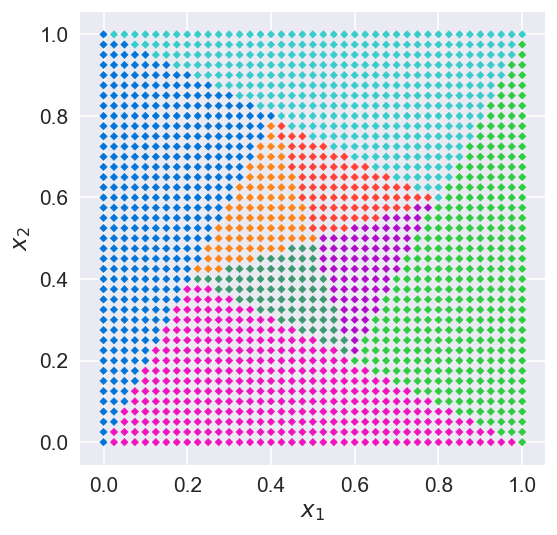
\includegraphics[width=\textwidth]{12}
		\caption{Выборка на плоскости}
		\label{fig:eight_classes_sample}
	\end{subfigure}
	\caption{Разбиение и выборка на плоскости}
\end{center}
\end{figure}
\vspace{-1.5cm}

\subsection{Задание 3}

Исказим сформированную ранее выборку $(P, T)$, изменив значение $10\%$ случайно выбранных строк $T$ на случайные значения от 1 до 8, и будем интерпретировать эти данные, как ответ $Y$ некоторого распознающего устройства (классификатора). На рис. \ref{fig:eight_classes_noise} изображена полученная выборка $(P, Y)$.

\begin{figure}[H]
\begin{center}
	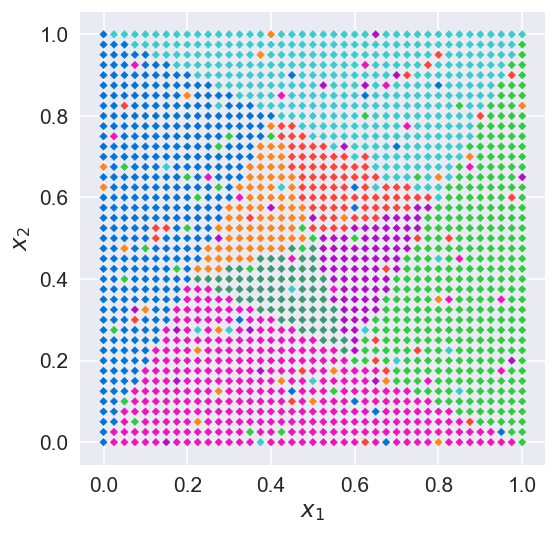
\includegraphics[scale=1]{13}
	\caption{Выборка, содержащая ошибки}
	\label{fig:eight_classes_noise}
\end{center}
\end{figure}

На основании желаемых $T$ и реальных $Y$ ответов определим основные показатели качества распознавания. На рис. \ref{fig:eight_classes_conf_matrix} изображена матрица неточностей.

\begin{figure}[H]
\begin{center}
	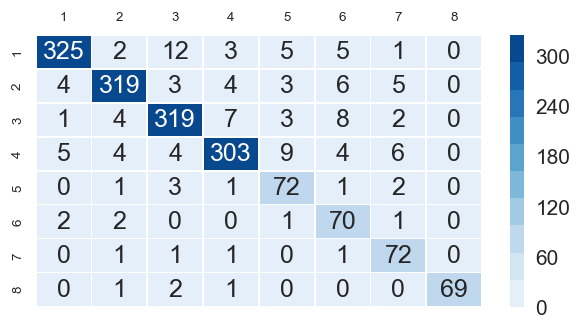
\includegraphics[scale=1]{14}
	\caption{Матрица неточностей}
	\label{fig:eight_classes_conf_matrix}
\end{center}
\end{figure}

По значениям матрицы неточностей найдем другие характеристики классификации:
\begin{itemize}
	\setlength\itemsep{0em}
	\item Средняя вероятность ошибки: $0.08$
	\item Средняя вероятность правильного распознавания: $0.92$
\end{itemize}

В таблице \ref{tab:eight_classes_errors} указаны значения ошибок первого и второго рода для каждого класса.

\vspace{-0.5cm}
\begin{table}[H]
\begin{center}
	\begin{tabular}{|c|c|c|c|c|c|c|c|c|}
		\hline
		Ошибка\textbackslash класс & 1 & 2 & 3 & 4 & 5 & 6 & 7 & 8 \\ 
		\hline
		1 род & 0.04 & 0.05 & 0.08 & 0.06 & 0.29 & 0.36 & 0.24 & 0.00 \\ 
		\hline
		2 род & 0.09 & 0.08 & 0.08 & 0.11 & 0.11 & 0.09 & 0.06 & 0.06 \\ 
		\hline
	\end{tabular}
	\caption{Ошибки первого и второго рода}
	\label{tab:eight_classes_errors}
\end{center}
\end{table}

\section{Непрерывная функция одной переменной}

\subsection{Задание 1}

Определим функцию одной переменной в интервале входных значений $x \in [0, 1]$, имеющую несколько экстремумов и колебания различной частоты. Функция изображена на рис. \ref{fig:function}.

\begin{figure}[H]
\begin{center}
	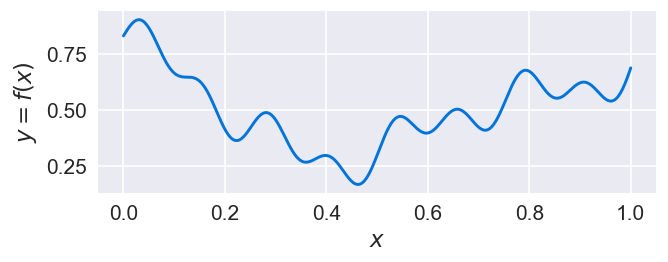
\includegraphics[scale=1]{15}
	\caption{Непрерывная функция}
	\label{fig:function}
\end{center}
\end{figure}

\subsection{Задание 2}

Сформируем множество входных значений $P$ в диапазоне возможных значений функции и определим соответствующие значения $T$. Полученная выборка изображена на рис. \ref{fig:function_sample}.

\begin{figure}[H]
\begin{center}
	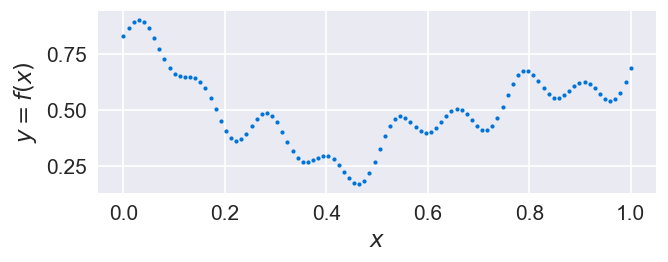
\includegraphics[scale=1]{16}
	\caption{Выборка значений непрерывной функции}
	\label{fig:function_sample}
\end{center}
\end{figure}

\subsection{Задание 3}

Добавим к значениям $T$ равномерный шум амплитуды, равной 10\% от максимального значения. Будем интерпретировать полученный сигнал, как ответ $Y$ некоторого распознающего устройства (нейронной сети).

\begin{figure}[H]
\begin{center}
	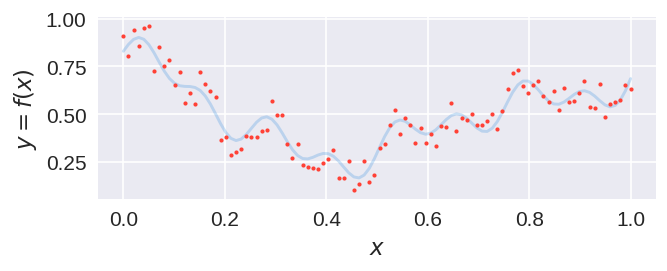
\includegraphics[scale=1]{17}
	\caption{Зашумленная непрерывная функция}
	\label{fig:function_noise}
\end{center}
\end{figure}

На основании желаемых $T$ и реальных $Y$ ответов определим основные показатели качества распознавания:
\begin{itemize}
	\setlength\itemsep{0em}
	\item Средняя абсолютная ошибка: $0.0506$
	\item Средняя относительная ошибка: $0.1276$
	\item Максимальная по модулю ошибка: $0.0994$
\end{itemize}

\newpage

\section{Линейная функция с памятью}

\subsection{Задание 1}

Зададим линейную функция с памятью:
\begin{equation*}
y[n] = \sum_{i=0}^{h-1} x[n - i\cdot d]\cdot k_i,
\end{equation*}
где $h$ – ширина окна, $d$ – глубина задержек, $k_i$ – коэффициенты.

Зададим коэффициенты: $h = 8, d = 4$,\\
$k_i = [0.183, -0.826, 0.286, -0.927, 0.970, -0.571, -0.143, -0.375]$.

\subsection{Задание 2}

Подадим несколько вариантов входных сигналов: гармонический, ступенчато изменяющийся и случайный. Сформированные входные (синим цветом) и выходные (красным цветом) сигналы изображены на рис. \ref{fig:linear_function}.

\begin{figure}[H]
\begin{center}
	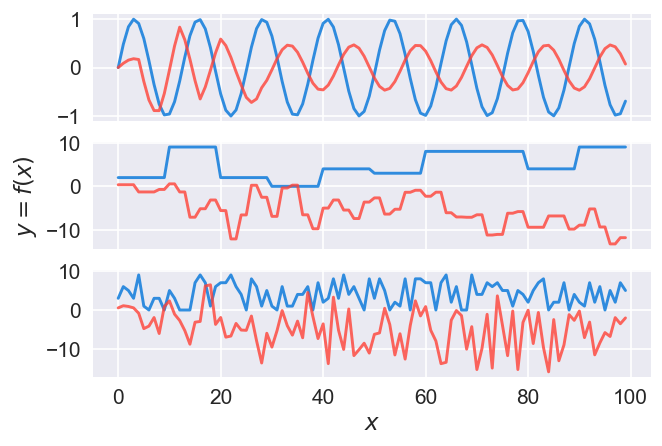
\includegraphics[scale=1]{18}
	\caption{Входной и выходной сигнал линейной функции с памятью}
	\label{fig:linear_function}
\end{center}
\end{figure}

\section{Нелинейная функция с памятью}

\subsection{Задание 1}

Зададим нелинейную функцию с памятью:
\begin{equation*}
y[n] = f(x[n], x[n - d],..., x[n - (h - 1)\cdot d]),
\end{equation*}
где $h$ – ширина окна, $d$ – глубина задержек.

Зададим функцию: $f(x_1, x_2,...,x_n) = \sqrt{x_1^2 + x_2^2 + ... + x_n^2}$.

Зададим коэффициенты: $h = 3, d = 2$.

\subsection{Задание 2}

Подадим несколько вариантов входных сигналов: гармонический, ступенчато изменяющийся и случайный. Сформированные входные (синим цветом) и выходные (красным цветом) сигналы изображены на рис. \ref{fig:non_linear_function}.

\begin{figure}[H]
\begin{center}
	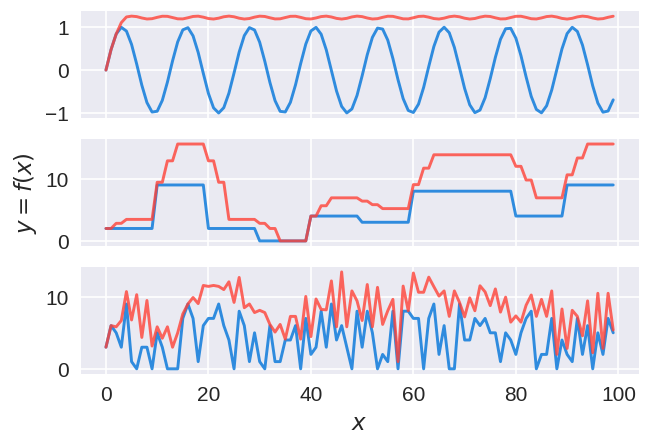
\includegraphics[scale=1]{19}
	\caption{Входной и выходной сигнал нелинейной функции с памятью}
	\label{fig:non_linear_function}
\end{center}
\end{figure}

\newpage

\section{Линейное разностное уравнение}

\subsection{Задание 1}

Зададим линейное разностное уравнение 
\begin{equation*}
y[n] = (z_1 + z_2) \cdot y[n-1] - z_1 \cdot z_2 \cdot y[n-2] + k_1 \cdot X[n] + k_2 \cdot X[n-1]
\end{equation*}
где $z_1, z_2, k_1, k_2$ – некоторые коэффициенты.

Зададим коэффициенты: $z_1 = 0.5, z_2 = -0.5, k_1 = 0.25, k_2 = 0.5$.

\subsection{Задание 2}

Подадим несколько вариантов входных сигналов: гармонический, ступенчато изменяющийся и случайный. Сформированные входные (синим цветом) и выходные (красным цветом) сигналы изображены на рис. \ref{fig:difference_equation}.

\begin{figure}[H]
\begin{center}
	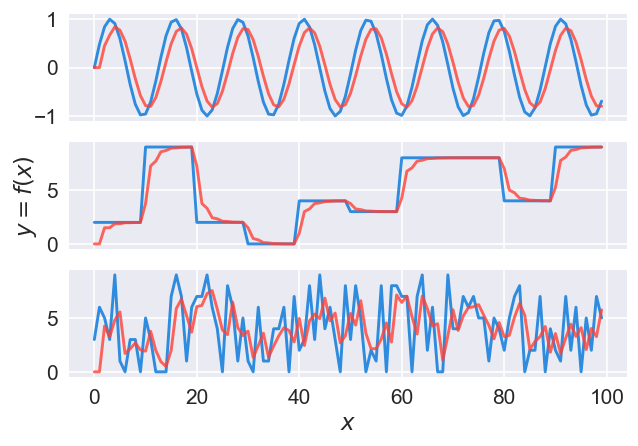
\includegraphics[scale=1]{20}
	\caption{Входной и выходной сигнал линейного разностного уравнения}
	\label{fig:difference_equation}
\end{center}
\end{figure}

\newpage

\section{Многомерные образы}

\subsection{Задание 1}

Для задачи классификации будем использовать набор, встроенный в библиотеку \textbf{scikit} для языка программирования Python. Набор включает в себя 1797 черно-белых изображений рукописных цифр (то есть 10 классов) размером $8 \times 8$ пикселей.

\subsection{Задание 2}

На рис \ref{fig:digits} изображены примеры образов каждого класса.

\begin{figure}[H]
\begin{center}
	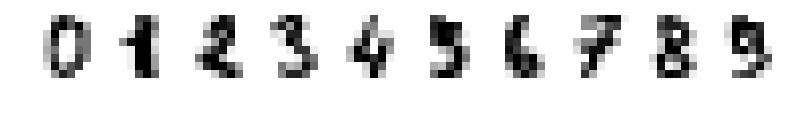
\includegraphics[scale=1]{21}
	\caption{Примеры образов каждого класса}
	\label{fig:digits}
\end{center}
\end{figure}

На рис. \ref{fig:digits_noise} изображены примеры образов, зашумленных с разной степенью интенсивности относительно исходных.

\begin{figure}[H]
\begin{center}
	\begin{subfigure}[b]{\textwidth}
		
\includegraphics[width=\textwidth]{22}
	\end{subfigure}
	\begin{subfigure}[b]{\textwidth}
		
\includegraphics[width=\textwidth]{23}
	\end{subfigure}
	\begin{subfigure}[b]{\textwidth}
		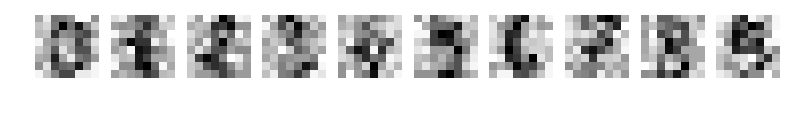
\includegraphics[width=\textwidth]{24}
	\end{subfigure}
	\caption{Зашумленные образы каждого класса}
	\label{fig:digits_noise}
\end{center}
\end{figure}

\newpage

На рис \ref{fig:digits_rotation} изображены примеры образов, имеющих геометрические искажения (поворот на различный угол).

\begin{figure}[H]
\begin{center}
	\begin{subfigure}[b]{\textwidth}
		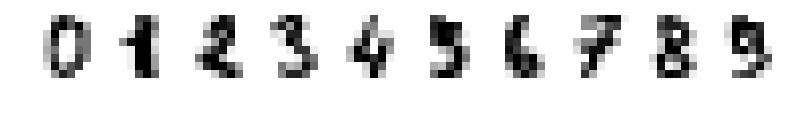
\includegraphics[width=\textwidth]{25}
	\end{subfigure}
	\begin{subfigure}[b]{\textwidth}
		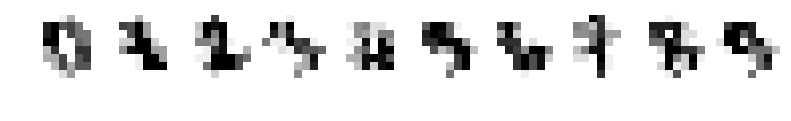
\includegraphics[width=\textwidth]{26}
	\end{subfigure}
	\begin{subfigure}[b]{\textwidth}
		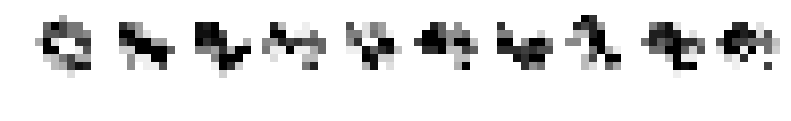
\includegraphics[width=\textwidth]{27}
	\end{subfigure}
	\begin{subfigure}[b]{\textwidth}
		
\includegraphics[width=\textwidth]{28}
	\end{subfigure}
	\caption{Повороты на различный угол образов каждого класса}
	\label{fig:digits_rotation}
\end{center}
\end{figure}

На рис \ref{fig:digits_part} изображены образы, являющиеся некоторой частью от исходных.

\begin{figure}[H]
\begin{center}
	
\includegraphics[scale=1]{29}
	\caption{Примеры искаженных образов каждого класса}
	\label{fig:digits_part}
\end{center}
\end{figure}

\end{document}